\documentclass[usenames,dvipsnames,pdf]{beamer}

\usepackage{textcomp}
\usepackage{pifont}
\usepackage[utf8]{inputenc}
\usepackage{amsfonts}
\usepackage{amstext}
\usepackage{amsmath}
\usepackage{fancyhdr}
\usepackage{amsthm}
\usepackage{epsfig}
\usepackage{graphicx}
\usepackage{multicol}
\usepackage{cite}
\usepackage{natbib}
\usepackage{adjustbox}
\usepackage{bussproofs}
\usepackage{stmaryrd}
\usepackage[tableaux]{prooftrees}
\usepackage{qtree}
\usepackage{mathtools}
\usepackage{scalerel,stackengine}
\usepackage[all]{xy}
% \usetikzlibrary{automata, positioning, shapes, arrows}
% \usepackage[dvipsnames]{xcolor}

\usetheme{CambridgeUS}

%\useoutertheme{miniframes} % Alternatively: miniframes, infolines, split
%\useinnertheme{circles}

%\definecolor{UBCblue}{rgb}{0.04706, 0.13725, 0.26667} % UBC Blue (primary)

% \usecolortheme[named=UBCblue]{structure}
% \usecolortheme[named=RoyalBlue]{structure}
\usecolortheme{seahorse}

% \usecolortheme{beaver}
%\setbeamercolor{spruce}{fg=cyan!90!black}

%\setbeamertemplate{itemize item}{\color{teal}$\blacktriangleright$}
%\setbeamertemplate{itemize subitem}{\color{teal}$\blacktriangleright$}

\renewcommand{\phi}{\varphi}

\graphicspath{ {./images/} }


% \newcommand{\newState}[4]{\node[state,#3](#1)[#4]{#2};}
% \newcommand{\newTransition}[4]{\path[->] (#1) edge [#4] node {#3} (#2);} 
\renewcommand*\linenumberstyle[1]{(#1)}
\def\apeqA{\SavedStyle\sim}
\def\apeq{\setstackgap{L}{\dimexpr.5pt+1.5\LMpt}\ensurestackMath{%
  \ThisStyle{\mathrel{\Centerstack{{\apeqA} {\apeqA}}}}}}

\def\dis{\displaystyle}

\def\QQ{\mathbb Q}
\def\ZZ{\mathbb Z}
\def\RR{\mathbb R}
\def\CC{\mathbb C}
\def\FF{\mathbb F}
\def\NN{\mathbb N}
\def\AA{\mathbb A}
\def\II{\mathbb I}

\def\Cc{\mathcal C}
\def\Dd{\mathcal D}
\def\Pp{\mathcal P}

\def\Af{\mathfrak A}
\def\Bf{\mathfrak B}
\def\Cf{\mathfrak C}
\def\Df{\mathfrak D}
\def\Ef{\mathfrak E}
\def\Ff{\mathfrak F}
\def\Gf{\mathfrak G}
\def\Hf{\mathfrak H}
  
% define 2x2 matrix:
\newcommand\twodmatrix[4]{ \ensuremath{ \left( 
	\begin{array}{cc}
		#1 & #2  \\
		#3 & #4 
	\end{array}  
	\right) } }
  

%%%%%%%%%%%%%%%%%%%%%%%%%%%%%%%%%%%%%%%%%%%%%
\setbeamerfont{footnote}{size=\tiny}

\DeclareMathSymbol{:}{\mathord}{operators}{"3A}

\mode<presentation>{}
%% preamble
\title{A sequence-to-sequence approach for document-level relation extraction}
\author{John Giorgi, Gary D. Bader, Bo Wang}
\begin{document}
	%% title frame
	\begin{frame}
		\titlepage
	\end{frame}


        \section{Overview}

        \begin{frame}{Introduction}
          \begin{itemize}
          \item
            Novel end-to-end joint learning approach for inter-sentence relation extraction.\footnote{Document-level is a stretch, due to encoder limit of 512 tokens they did paragraphs.}
          \item
            Utilizes sequence to sequence architecture.
          \item
            Representation schema for coreferent entities, $n$-ary relations, and disjoint spans in output.
          \end{itemize}
        \end{frame}

        \begin{frame}{Introduction}
          \begin{itemize}
          \item
            New benchmarks for end-to-end results over some biomedical datasets.
          \item
            Competitive results against more complex architectures for datasets with established end-to-end results.
          \end{itemize}
        \end{frame}

        \begin{frame}{Defining Terms}
          End-to-end RE:
          \begin{itemize}
          \item
            Relation extraction depends on entities.
          \item
            Pipeline methods (current standard), use one or more models for NER, and one or more models for RE over discovered entities.
          \item
            End-to-end approaches use one model (possibly with a classification head) to discover the relations,
            relying on internal representations to jointly extract and implicitly coordinate entity and relation information.
          \end{itemize}

          \textbf{NB:}  The authors use \textit{pipeline} to refer to the RE component.
          In NER/RE practice, pipeline usually refers to the whole system, NER component included.  
        \end{frame}

        \begin{frame}{Defining Terms}
          Coreference:
          \begin{itemize}
          \item
            The same entity may have one or more mentions in a given text unit (type vs. token).
          \item
            If a relation holds between two entites, how to reflect this for each entity's mentions?
          \end{itemize}
        \end{frame}
        
        \begin{frame}{Motivation}
          \begin{itemize}
          \item
            Lots of entity and relation information at the document and cross document level.
          \item
            Generalizing sentential pipeline methods (the current standard) for inter-sentential RE is very tricky.\footnote{e.g. our NER/RE system for radiotherapy.}
          \item
            Lots of information takes the form of $n$-ary relations, tricky to reconstruct this from binary relations.
          \end{itemize}
        \end{frame}
        
        \section{Method}

        \begin{frame}{Linearization Schema}
          \begin{figure}
          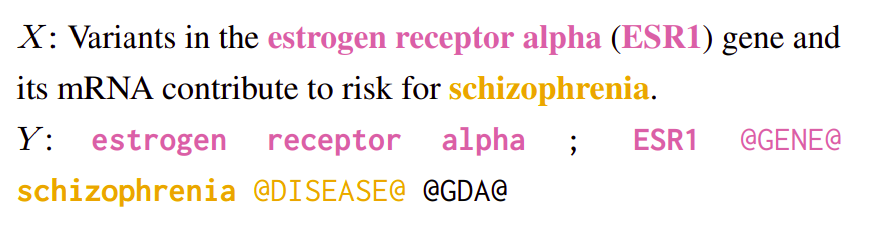
\includegraphics[width=0.7\textwidth,height=0.7\textheight,keepaspectratio]{linearization} 
          \end{figure}
          Schema is:

          
          \begin{adjustbox}{varwidth=\linewidth}%,scale=0.7}
            %% \begin{framed}
            %\centering
            \small\text{$<\textit{entity mention}_{1,1}>$ ; ... ; $<\textit{entity mention}_{1,n}>$ $<entity type_1> \dots$}


            \small\text{$<\textit{entity mention}_{m,1}>$ ; ... ; $<\textit{entity mention}_{m,k}>$ $<entity type_m>$}


            \small\text{$<relation type>$}
            \end{adjustbox}
        \end{frame}

        \begin{frame}{Model Structure}
          
        \end{frame}

        \begin{frame}{Evaluation}
          
        \end{frame}

        \begin{frame}{Simulating RE on Gold Entities (Entity Hinting)}
          \begin{figure}
            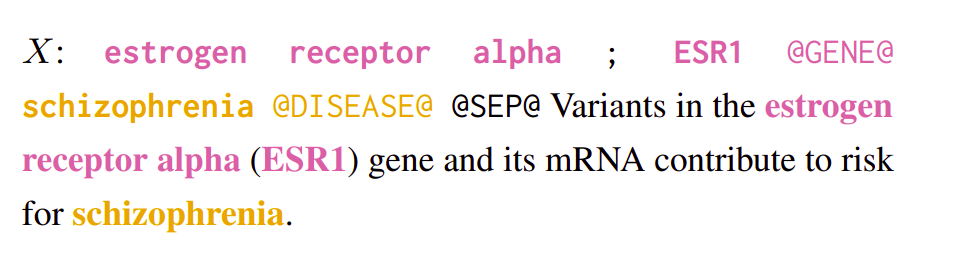
\includegraphics[width=0.7\textwidth,height=0.7\textheight,keepaspectratio]{entity_hint} 
          \end{figure}
        \end{frame}
        
        \section{Results}

        \begin{frame}{Datasets}
          \begin{itemize}
          \item \textbf{CDR}


            Chemical-induced disease (CID) relations.  Sentential 
          \item \textbf{GDA}


            Gene-disease associations.  Sentential    
          \item \textbf{DGM}

            Drug-gene-mutations.  Sentential
          \item \textbf{DocRED}
            General domain.  Inter-sentential/document-level
            
          \end{itemize}
        \end{frame}

        \begin{frame}{Datasets}
          CDR and GDA are annotated over PubMed titles and abstracts.
          DGM from PubMed articles.
          DocRED from Wikipedia. \hfill \break \hfill \break
          
          
          CDR and DocRED are manually annotated.
          Unfortunately GDA and DGM are generated via distant supervision.\hfill \break \hfill \break

        
          
          DocRED has a very rich taxonomy, 6 entity types and 96 relation types.
        \end{frame}

        
        \section{Analysis}


        \begin{frame}{$n$-ary Relations (DGM)}
          \begin{figure}
            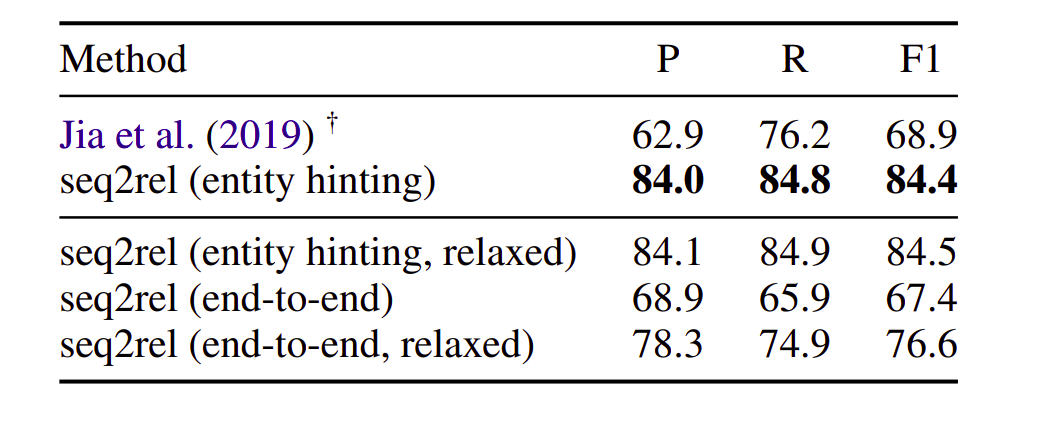
\includegraphics[width=0.7\textwidth,height=0.7\textheight,keepaspectratio]{DGM_n_ary_comparison} 
          \end{figure}
          DGM has ternary relations.
        \end{frame}

        \begin{frame}{RE with Gold Entities (CDR, GDA)}
          \begin{figure}
            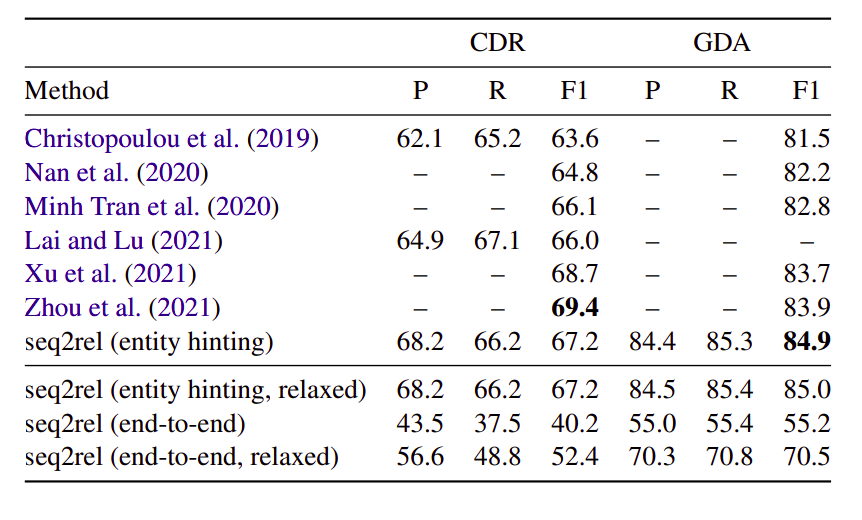
\includegraphics[width=0.7\textwidth,height=0.7\textheight,keepaspectratio]{CDR_GDA_gold_entities} 
          \end{figure}
        \end{frame}

        \begin{frame}{End-to-end RE (DocRED)}
          \begin{figure}
            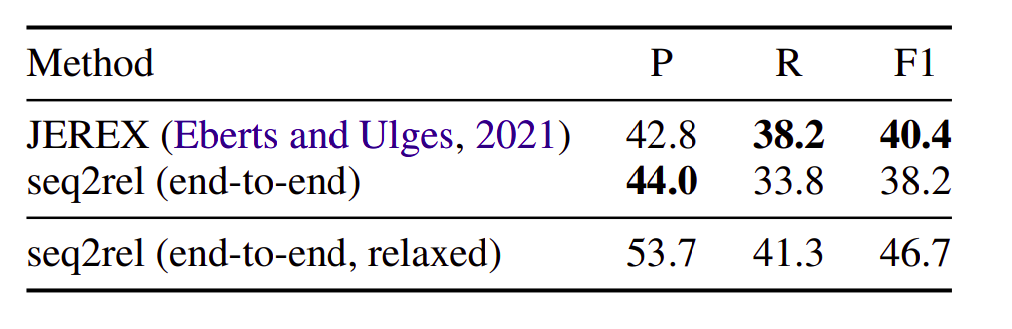
\includegraphics[width=0.7\textwidth,height=0.7\textheight,keepaspectratio]{DocRED_e2e_comparison} 
          \end{figure}
        \end{frame}


        \begin{frame}{End-to End RE Ablation (CDR, DocRED)}
          \begin{figure}
            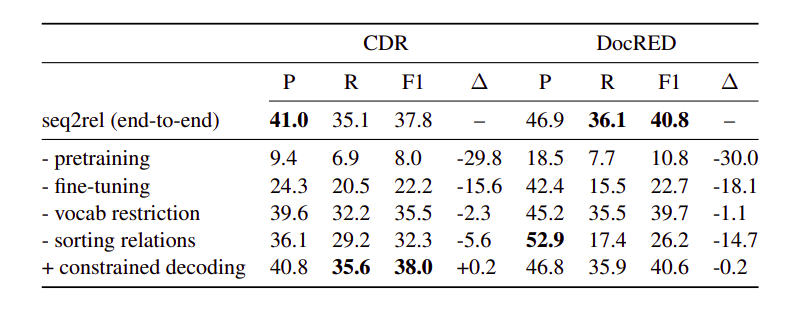
\includegraphics[width=0.7\textwidth,height=0.7\textheight,keepaspectratio]{ablation} 
          \end{figure}
        \end{frame}

        \begin{frame}{Training Set Size vs. Performance (CDR, GDA)}
          \begin{figure}
            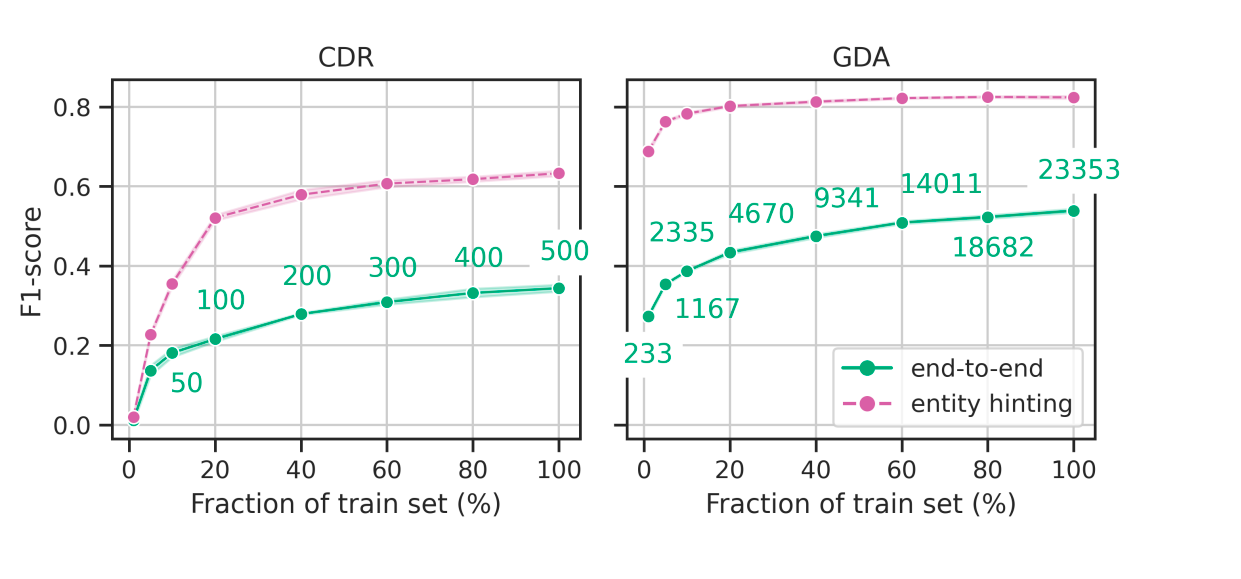
\includegraphics[width=0.7\textwidth,height=0.7\textheight,keepaspectratio]{training_set_size_plateau} 
          \end{figure}
        \end{frame}
        
        \section{Conclusion}

        \begin{frame}{Conclusion}
        \end{frame}

        \begin{frame}[allowframebreaks]
          \frametitle{References}
          \bibliographystyle{acl}
          %\nocite{quantified}
          %\nocite{hansen2007tableau} 
          %\nocite{bolander2009terminating}
          %\nocite{bolander2007termination}
          %\nocite{hungar1995if}
          %\nocite{bhat1998tableau}
          \bibliography{references}
        \end{frame}
      \end{document}
      
      
